\documentclass{article}
\usepackage{graphicx} % Required for the inclusion of images
\usepackage{natbib} %bibliography style 
\usepackage{amsmath} % Required for some math elements 
\usepackage{hyperref}
\usepackage{caption}
\usepackage{listings}
\usepackage{color} %red, green, blue, yellow, cyan, magenta, black, white
\definecolor{mygreen}{RGB}{28,172,0} % color values Red, Green, Blue
\definecolor{mylilas}{RGB}{170,55,241}
\definecolor{vblue}{RGB}{49,49,255}
\setlength{\parskip}{1em}
\setlength{\parindent}{0pt}
\usepackage{setspace}
\usepackage[margin=1in]{geometry}
\usepackage[T1]{fontenc} % optional
\usepackage{tgtermes}
\renewcommand{\labelenumi}{\alph{enumi}.}
%bibliography style 
\usepackage[style=ieee]{biblatex}
\addbibresource{bib.bib}
\DeclareLanguageMapping{english}{ieee}

%%TITLE PAGE
\linespread{1.3}

\lstset{language=Python,%
    basicstyle=\footnotesize\ttfamily,breaklines=true,
    breaklines=true,%
    morekeywords={matlab2tikz},
    keywordstyle=\color{vblue},%
    morekeywords=[2]{1}, keywordstyle=[2]{\color{black}},
    identifierstyle=\color{black},%
    stringstyle=\color{mylilas},
    commentstyle=\color{mygreen},%
    showstringspaces=false,%without this there will be a symbol in the places where there is a space
    numbers=left,%
    numberstyle={\tiny \color{black}},% size of the numbers
    numbersep=9pt, % this defines how far the numbers are from the text
    emph=[1]{for,end,break},emphstyle=[1]\color{red}, %some words to emphasise
    %emph=
    }
\renewcommand{\labelenumi}{\alph{enumi}.} % Make numbering in the enumerate environment by letter rather than number (e.g. section 6)

\title{The University of British Columbia Okanagan
School of Engineering \\ \vspace{1cm} ENGR 453 \\
Cloud Project Proposal \vspace{2cm}} % Title
\date{Submitted: April \(23^{rd}\), 2020  \vspace{2cm}} % Date for the report
\author{Student \#1 Name: Graeme \textsc{Paul}\\
Student \#2 Name: Daara \textsc{Abbassi-Mohadjel}} % Author name

\begin{document}
\maketitle
%\newpage
%\tableofcontents

%\newpage
\clearpage
\section{Proposal \& Introduction}
For our cloud project, there will be three devices which will work together to control the Raspberry Pi as it records a temperature and controls a heating lamp. The purpose of the project is to 'cure' a composite which is in a curing oven. The internal temperature of the part is indeterminable thus it is unknown how long the part is required to cure. Figure 1 shows the typical heating curve of an object in the curing oven. A machine learning algorithm has been trained with the internal temperature data from similar composite parts thus by knowing the air temperature and current time the internal temperature of the current part can be found. A Raspberry Pi recording time and air temperature will be used with a machine learning algorithm on the cloud virtual machine which will make a prediction when to stop the Raspberry Pi.
\begin{figure}[h]
    \centering
    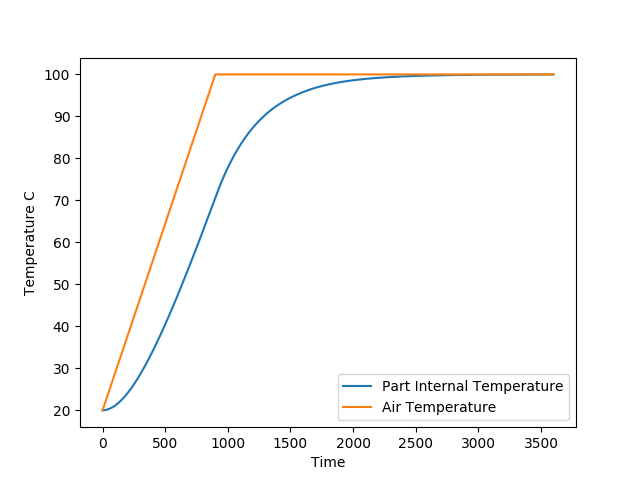
\includegraphics[width=.5\textwidth]{Figure_1.png}
    \caption{Heating Curve of Composite Part in Curing Oven}
    \label{fig:curveplot}
\end{figure}
\newpage
The full cycle of data is as follows. First, the local PC will be the initial stimulus of the system. When a start command is sent using MQTT, the cloud will act on this and initiate the Raspberry Pi to start heating the oven and recording air temperature and time. The collected data will be sent to the virtual machine. A prediction is done by the virtual machine using the temperature data halfway through the run and is used to determine a reasonable stop time. The Raspberry Pi will be told to stop by the virtual machine and the run data and prediction will be sent back to the control PC for review. A summary of this data flow is shown in Figure 2.
\begin{figure}
    \centering
    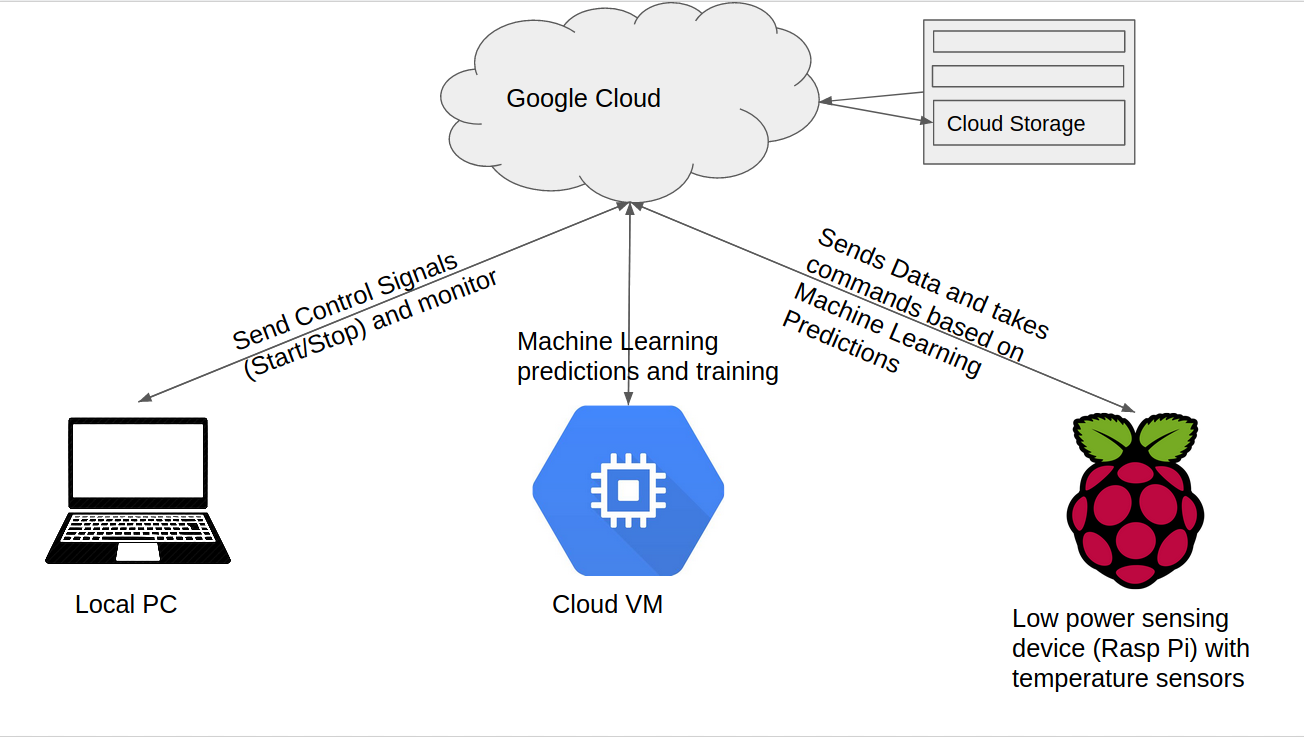
\includegraphics[width=.9\textwidth]{cloud.png}
    \caption{Data flow the IOT network}
\end{figure}
\newline

Additional notes:\\
Due to circumstances and no access to real data the system is using machine generated data which is essentially equivalent. No Raspberry Pi will be used but instead just another computer which will act as the Raspberry Pi and no temperature sensors will be used as neither group member has access to the equipment. Essentially, the cloud framework will be developed to show a proof of concept that control of the device is possible over the cloud. 
\newpage
\section{Design}
There were a number of considerations taken into account for the design of this project and are discussed below. For a video summary of the working deign see Section \ref{example_perf} Example of Performance.
\subsection{Data Payload}
The payload that is communicated between the devices, the virtual machine data logger and the cloud virtual machine, contain several pieces of information necessary for generating a prediction. A message sent as \lstinline{data_payload} is sent as a dictionary seen from the line of code below, there are four keys in the dictionary. 
\begin{lstlisting}
data_payload = json.dumps(\{"Type": TYPE, "Data" :DATA, "Time" : TIME, "To" : DEVICE\})
\end{lstlisting}
First is the \lstinline{"Type"} which signifies an update of the state for a device if set to 1 ,and when set to 0 it will signify temperature or air data for the virtual machine or control computer.  Another item in the payload is the \lstinline{"Time"}, which returns time at the instances payloads are sent throughout the process. The \lstinline{"Data"} key corresponds to data that is used to run the process, such as sending the starting temperature and the stop time to the Raspberry Pi. The last key \lstinline{"To"} is for setting the destination device for the payload to be sent to. The \lstinline{"To"} flag is only used by the cloud to direct messages to the correct device. The below code shows an example of the VM acting on data that it is receiving, first it determines if the message is data or a configuration update by checking the \lstinline{"Type"}, then it extracts the data from the \lstinline{"Data"} key. It can be seen that some configurations include to start predicting, to stop/done and to reset. 
\lstinputlisting[language=Python, linerange={225-251}]{vm_mqtt_code.py} 
 \medskip


%-payload has type 1 for device configuration, 0 for data
%-payload has time
%-payload has who it goes to
%-payload has data
%-uses json/dict format

\subsection{Data Collection and Data Processing} \label{data_collection} 
Once the Raspberry Pi receives the signal to begin the data collection process from the control PC, air temperature data is recorded from temperature sensors inside the heating chamber. For this project, we decided to have the Raspberry Pi send the temperature data in batches to the Cloud virtual machine so that the virtual machine may act on the data in real time. The Cloud virtual machine is storing the measurements from the Raspberry Pi into an array and checking for the temperature to reach steady state, and afterwards a set time will be sent back to the Raspberry Pi to arrange the moment the infrared lamp will turn off. The array index is also sent with each batch of data so that the data does not get disorganized, as there is no guarantee that the order that data is received is the order it was sent. The data collection process continues temporarily after the lamp is turned off because in a practical setting the temperature would then start to decrease, but as this is only a proof of concept, the temperature remains at steady state in our demonstration. 


%-Temp data sent in batches so VM can act on it in real time
%-array index sent with data so it doesn't get disorganized as there is no guarantee in order data is received
%-data>>vm>>prediciton

\subsection{Control Computer}
The control computer takes user input and is able to start, stop, or reset a test by updating the other devices configurations. The control computer also sets the run ID which makes it so that the saved data from the run is a unique filename when written to the cloud storage bucket. The control computer will receive the prediction and all of the collected air temperature at the end of the test so that it can be saved and plotted. Figure \ref{fig:curveplot} shown in the introduction is the output from this plotting feature. Below is the code which implements these features.
\lstinputlisting[language=Python, linerange={241-272}]{control_mqtt.py} 

\subsection{Prediction}
Keras was chosen for this project due to its accessibility in implementing machine learning algorithms using Tensorflow in Python. The machine learning algorithm used was a Long Short-term Memory (LSTM) neural network and the algorithm was trained using data generated in MATLAB. The predictions for the part temperature act off of the time and air temperature that is sent from the data logger outlined in Section \ref{data_collection}. Once the virtual machine detects the plateau of the air temperature, a prediction is then made for the part temperature and the data is stored. The code shown below is the prediction process. First the pre-trained Keras model is loaded, then the received data is scaled and used to predict.  
\lstinputlisting[language=Python, linerange={168-193}]{vm_mqtt_code.py} 

%-keras to predict
%-acts of time and air temp data
%-makes prediction when temp data plateaus

\subsection{Google Cloud}
In this project, all the devices use MQTT to connect to the Google Cloud device registry. The MQTT message goes to a Cloud Pub/Sub topic, therefore any message published to a topic is immediately received by all of the subscribers to the topic. The Pub/Sub messaging provides a simple and reliable staging location for the event data and acts to ingest events so that it can be acted upon. The Cloud Function will then act on the event data and can send messages to the devices through MQTT. We are able to implement any number of IoT devices using this system. Buckets are also used to permanently store data in the Cloud. 
\begin{figure}[h]
    \centering
    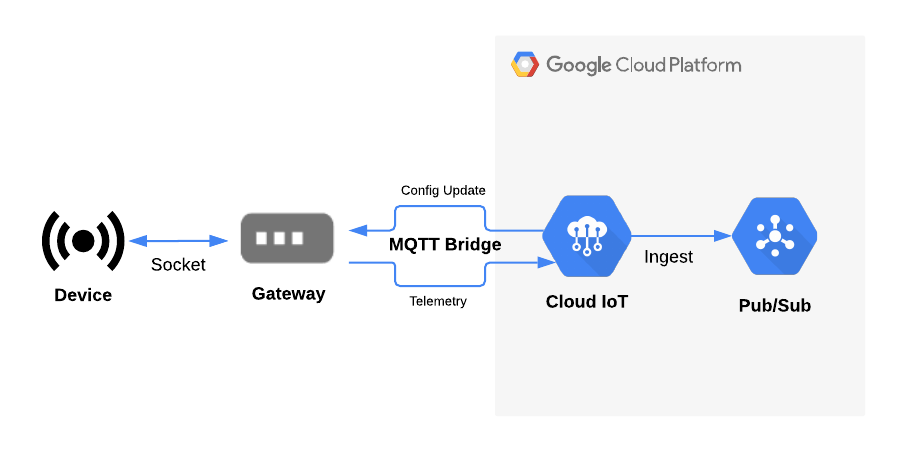
\includegraphics[width=\linewidth]{gateway-arch.png}
    \caption{A Google Cloud Implementation}
    \label{fig:gcloud}
\end{figure}
%-Devices all use mqtt to connect to their google cloud device registry
%-mqtt message goes to a pub/sub topic which acts as ingest for message so that it can be acted on 
%-cloud function acts on this data
\subsection{Code License}
As the code used for this project was modified and adapted from Google Cloud examples which were using the Apache license, we also needed to use the Apache License due to copyleft. 
%-modified from google cloud examples they used apache license because of copyleft we need to use apache license.

%-cloud function can send messages using google cloud to device using mqtt
%-bucket is used to permanenetly store data
\subsection{Virtual Machine}
The Cloud virtual machine used in this project is a standard Linux virtual machine. The virtual machine from Google Cloud accelerates the prediction speed and allows the Raspberry Pi to continue to measure temperatures so that there is minimal data loss while a live prediction is made.
%-vm is pretty standard
%-used to accelerate prediction speed and allow temp device to read temps while prediction is made so minimal data is lost
\subsection{AWS vs Google Cloud Comparison}
There are a large number of differences between the Google Cloud service and AWS. AWS offers more than 200 services and is more feature-rich compared to Google Cloud. Google Cloud has the advantage in terms of flexibility with far greater opportunities for customization of compute instances compared to AWS. Furthermore, the Google Cloud platform has more advanced virtual machines than AWS. Lastly, Google Cloud had advantages in cost for the implementation of our project.
\subsection{Costs}
The costs for this project are primarily derived from leaving the virtual machine on in the Cloud, which resulted in roughly \$7 in costs. These costs were accumulated over multiple days of testing and validating the system, sending messages, and having the virtual machine on. This was not a concern as we had a complimentary \$350 dollars for use. 
%-costs mostly from just leaving virtual machine on around 7 dollars
%-got 350 dollars for free so not a big deal
\begin{figure}[h]
    \centering
    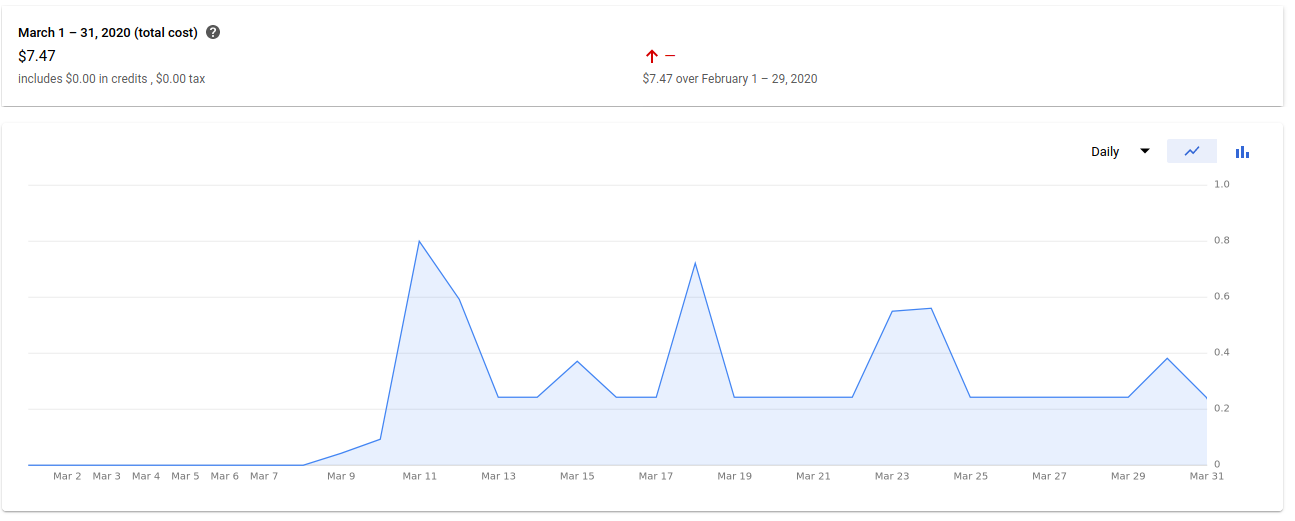
\includegraphics[width=.75\linewidth]{costs.png}
    \caption{Costs}
    \label{fig:costs}
\end{figure}
\newpage

\subsection{Implementation Assumption}
Due to limited access to the university's labs, we were unable to gain access to the heat chamber setup, so a Raspberry Pi was not actually used and is represented by a Linux terminal due to these restrictions and is used for demonstrative purposes and to make the demonstration video easier to show. For additional testing purposes, two separate computers were used a laptop and desktop and it was successful, therefore it should be able to work with a Raspberry Pi. 
%-no access to thermistors, second computer/raspberrypi so wasn't used

\section{Code Analysis}

\subsection{Device 1: Control Device}
The control device takes user input and can give a run an ID, or start/restart a run. The control device is also able to view a plot of the prediction and gathered run data. The main loop is shown in the code below.
\lstinputlisting[language=Python, linerange={241-273}]{control_mqtt.py}

\subsection{Device 2: Virtual Machine Device}
The virtual machine saves air temp data and predictions using the Google Cloud with the following functions shown below. The code snippet below shows the main loop which reads which state its in and performs actions based on it, including returning air and part temperatures, and saving the prediction it made.
\lstinputlisting[language=Python, linerange={362-404}]{vm_mqtt_code.py}
The code below shows how the virtual machine code loads a model file and the data it has collected to make a prediction in Keras.
\lstinputlisting[language=Python, linerange={168-193}]{vm_mqtt_code.py} 

\subsection{Device 3: Temp logger and Lamp control device}
The code below shows how the temp logger reads from a file (for lack of actual thermistors) and sends this data in batches to the virtual machine.
\lstinputlisting[language=Python, linerange={289-320}]{lamp_control_and_temp_log.py}
\subsection{Cloud Function}
The cloud function acts as the server and routes data to different devices. echo\_pubsub1 is executed whenever a message is published to the topic by any of the devices. 
\lstinputlisting[language=Python, linerange={15-35}]{cloud_function.py}

\section{Example of Performance} \label{example_perf}
Video of example: \href{https://www.youtube.com/watch?v=iKukfWf5Yn0&feature=youtu.be}{\textcolor{blue}{\underline{Video Demonstration.}}}
The video was cut before showing the saved prediction and collected data which is saved to the cloud storage bucket as a .CSV at the end of every run, but it can be seen that it was successful in the figure below.
\begin{figure}[h]
    \centering
    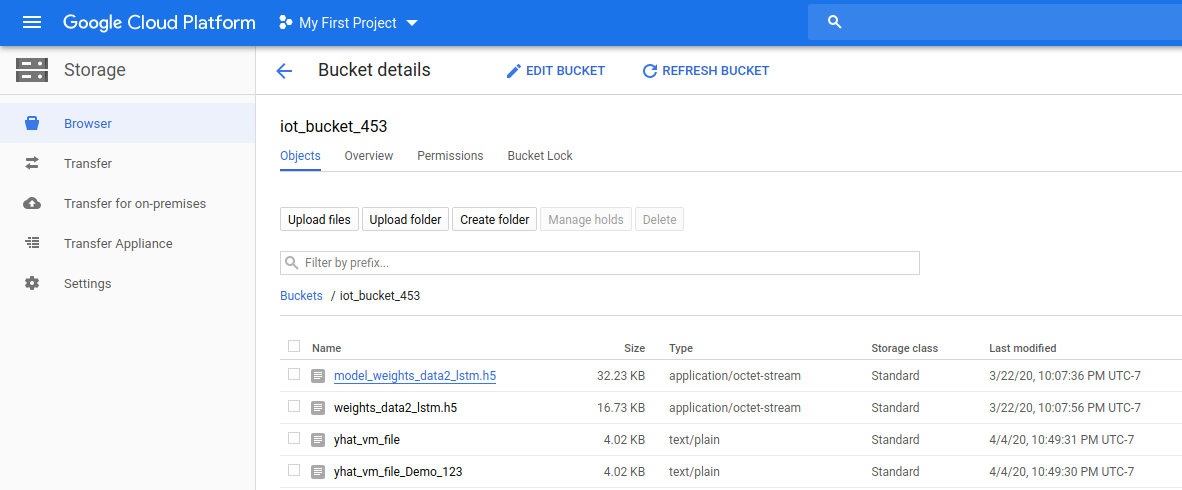
\includegraphics[width=.5\linewidth]{iot.png}
    \caption{Image showing saved prediction}
    \label{fig:iot_bucket}
\end{figure}
\\
link to github: \href{https://github.com/gaapaul/IotClassProject/tree/master/class_project}{\textcolor{blue}{\underline{github}}}
\section{Conclusion}
In this project, we were able to make use of the Google Cloud suite of cloud computing resources and services to implement a machine learning algorithm for a composite curing process. The goal of the project was accomplished by using MQTT communication between a Raspberry Pi for temperature measurements, a control PC, and a Google Cloud virtual machine for making a prediction for the part using an LSTM neural network. Ultimately, we were able to implement a data processing system with machine learning and an IoT network for composite curing.  
\section{Appendix}
\subsection*{Code}
\subsubsection*{Github Link}
link to github: \href{https://github.com/gaapaul/IotClassProject/tree/master/class_project}{\textcolor{blue}{\underline{github}}}
\subsubsection*{Control Device}
\lstinputlisting[language=Python]{control_mqtt.py}
\subsubsection*{VM Device}
\lstinputlisting[language=Python]{vm_mqtt_code.py}
\subsubsection*{Logger Device}
\lstinputlisting[language=Python]{lamp_control_and_temp_log.py}
\subsubsection*{Cloud function}
\lstinputlisting[language=Python]{cloud_function.py}

\printbibliography

\end{document}



